\documentclass[handout]{beamer}
% \documentclass{beamer}

%%
%%
%%
% From http://tex.stackexchange.com/questions/2072/beamer-navigation-circles-without-subsections
% Solution #2 or 3:
% \usepackage{etoolbox}
% \makeatletter
% % replace the subsection number test with a test that always returns true
% \patchcmd{\slideentry}{\ifnum#2>0}{\ifnum2>0}{}{\@error{unable to patch}}%
% \makeatother
% Solution #1:
\usepackage{remreset}% tiny package containing just the \@removefromreset command
\makeatletter
\@removefromreset{subsection}{section}
\makeatother
\setcounter{subsection}{1}


\usepackage{etex}
\usepackage{pgf}
\usepackage{tikz}
\usepackage{url}
\usepackage{amsmath}
\usepackage{color}
% \definecolor{red}{rgb}{1,0,0}
\usepackage{ulem}
% \usepackage{booktabs}
\usepackage{colortbl,booktabs}
\renewcommand*{\thefootnote}{\fnsymbol{footnote}}
\usepackage{fancybox}
\usepackage[framemethod=TikZ]{mdframed}
\mdfdefinestyle{FactStyle}{%
  outerlinewidth=0.5,
  roundcorner=1pt,
  leftmargin=1cm,
  linecolor=blue,
  outerlinecolor=blue!70!black,
  backgroundcolor=yellow!40
}
\usepackage{cancel}

  \newcommand\Warning{%
    \makebox[2.4em][c]{%
      \makebox[0pt][c]{\raisebox{.2em}{\Large!}}%
      \makebox[0pt][c]{\color{red}\Huge$\bigtriangleup$}}}%

\usepackage{stackengine}
\usepackage{scalerel}
\usepackage{xcolor}
  \newcommand\dangersign[1][2ex]{%
    \renewcommand\stacktype{L}%
    \scaleto{\stackon[1.3pt]{\color{red}$\triangle$}{\tiny !}}{#1}%
  }



\usepackage{dcolumn}
\newcolumntype{d}[1]{D{.}{.}{#1}}

% From
% http://tex.stackexchange.com/questions/109900/how-can-i-box-multiple-aligned-equations
\usepackage{empheq}
\usepackage{tcolorbox}  \newtcbox{\othermathbox}[1][]{%
  nobeforeafter, tcbox raise base, 
  colback=black!10, colframe=red!30, 
  left=1em, top=0.5em, right=1em, bottom=0.5em}

\newcommand\blue{\color{blue}}
\newcommand\red{\color{red}}
\newcommand\green{\color{green!75!black}}
\newcommand\purple{\color{purple}}
\newcommand\bluegreen{\color{blue!75!green}}
\newcommand\orange{\color{orange}}
\newcommand\redgreen{\color{red!50!green}}
\newcommand\grey{\color{black}}
\newcommand\gap{\vspace{.1in}}
\newcommand\nb{${\red\bullet}\ $}
\newcommand\halfgap{\vspace{.05in}}
\newcommand\divideline{\line(1,0){352}}
\usepackage{marvosym} % for \Smiley

\newcommand{\bluealert}[1]{{\blue\textbf{#1}}}

% \usepackage{beamerthemesplit} %Key package for beamer
\usetheme{Singapore}
% \usetheme{Szeged}
% \usetheme{Garfield}
% \usetheme{CambridgeUS}
% \usenavigationsymbolstemplate{} %Gets rid of slide navigation symbols


\setbeamercolor{separation line}{use=structure,bg=structure.fg!50!bg}
% \begin{beamercolorbox}[colsep=0.5pt]
%   {upper separation line foot}
% \end{beamercolorbox}



\makeatletter
\setbeamertemplate{footline}
{
  \leavevmode%
  \hbox{%
% \begin{beamercolorbox}[colsep=0.5pt]
%   {upper separation line foot}
% \end{beamercolorbox}


  \begin{beamercolorbox}[wd=.5\paperwidth,ht=2.25ex,dp=2ex,colsep=0.5pt]%
    {upper separation line foot}
    \usebeamerfont{author in head/foot}%
    \hspace*{2ex}\insertshortdate:\ \insertshorttitle
  \end{beamercolorbox}%
  \begin{beamercolorbox}[wd=.5\paperwidth,ht=2.25ex,dp=2ex,right]{title in head/foot}%
    \usebeamerfont{title in head/foot}
    {\insertshortauthor}\hspace*{2ex}
  \end{beamercolorbox}}%
  % \begin{beamercolorbox}[wd=.333333\paperwidth,ht=2.25ex,dp=2ex,right]{date in head/foot}%
  %   \usebeamerfont{date in head/foot}\insertshortdate{}\hspace*{2em}
  %   \insertframenumber{} / \inserttotalframenumber\hspace*{2ex} 
  % \end{beamercolorbox}%
  \vskip0pt%
}
\makeatother

\usetikzlibrary{decorations.markings}
\usetikzlibrary{arrows}


\title{Final Exam Review}
\author{Peter Garfield, UCSB Mathematics}
\date{March 15, 2017}
%\institute{}


\useinnertheme{default}

\usefonttheme{serif}
% \usecolortheme{rose}
% \usecolortheme{whale}
% \usecolortheme{orchid}
\usecolortheme{crane}
% \usecolortheme{dolphin}


%TEMPLATE
\setbeamertemplate{navigation symbols}{}

\setbeamertemplate{note page}[compress]

\setbeamertemplate{frametitle}{
  \vspace{0.5em}
  % \begin{centering}
  {\huge\blue\textbf{\textmd{\insertframetitle}}}
  \par
  % \end{centering}
}

% From http://tex.stackexchange.com/questions/7032/good-way-to-make-textcircled-numbers:
\newcommand*\circled[1]{\tikz[baseline=(char.base)]{\node[shape=circle,draw,fill=orange,inner sep=1pt] (char) {#1};}} 
% \renewcommand{\labelenumi}{\circled{\textbf{\arabic{enumi}}}}

\let\olddescription\description
\let\oldenddescription\enddescription
\usepackage{enumitem}
\let\description\olddescription
\let\enddescription\oldenddescription

% \usepackage[loadonly]{enumitem}
\setlist[enumerate,1]{label=\colorbox{orange}{\arabic*.},font=\bfseries}
%\setlist[enumerate,2]{label=\colorbox{blue!25}{(\alph*)},font=\bfseries}
% \setlist[enumerate,1]{label=\arabic*.,font=\bfseries}
\setlist[itemize,1]{label=\red$\bullet$}
\setlist[itemize,2]{label=\blue$\bullet$}

\newcommand\answer[1]{\fbox{#1}}
% \renewcommand\answer[1]{}

\newcommand{\antilog}{\operatorname{antilog}}







\title{}
\title{Calculus!}
\date{May 8, 2017}


\begin{document}
\small

\section*{Administration}

\frame{
  \frametitle{Office Hours!}
  % \ \vspace*{0.25in}

  {\Large{}Instructor:}\\
  \ \hspace*{0.2in} Trevor Klar, \url{trevorklar@math.ucsb.edu}\\[0.25em]

  {\Large{}Office Hours:}\\
  \ \hspace*{0.2in} Mondays 2--3\textsc{pm}, {\red{}Today 3--4pm}\\
  \ \hspace*{0.2in} Tuesdays 10:30--11:30\textsc{am}, {\red{}Tomorrow 3--4pm}\\
  \ \hspace*{0.2in} Thursdays 1--2\textsc{pm}\\
  \ \hspace*{0.2in} or by appointment \\[0.25em]

  {\Large{}Office:}\\
  \ \hspace*{0.2in} South Hall 6431X (Grad Tower, 6th floor, blue side, first door on the right)\\[0.5em]

  \copyright\ 2017\ Daryl Cooper, Trevor Klar

  % \vspace*{2in}
}


\section{Calculus Ideas}

\frame{
  \frametitle{Derivatives \&\ Differential Calculus}
  \ldots{}are about {\red how quickly things change}.
  % \gap

  \begin{itemize}
    \item Need to understand PRACTICAL significance in various
      situations
      \smallskip

      Spread of infectious disease, population growth, speed,
      acceleration, marginal rates in economics, global warming
      \medskip
      \pause

    \item {\blue Calculate (or estimate) rate of change}\ from various sources:
      \smallskip

      {\red graph}\\ 
      {\red table of data}\\ 
      {\red formula}
      \medskip
      \pause

    \item Applications: 
      \smallskip

      {\red measure change}\\ 
      {\red predict the future}\\  
      {\red optimization} -- find the best, or smallest, or biggest, or most\ldots\\ 
      \pause

  \end{itemize}
  %
  This is all about {\red\it{understanding}}\ the world.

}

\frame{
  \frametitle{Philosophical problem}

  How quickly is something changing at {\blue one moment}\ in time?
  \gap

  \uncover<2->{%
    Example: Does a ball {\red{}stop}\ when I throw it straight up?
  }
  \medskip

  \uncover<3->{%
    Example: How fast is the temperature rising at 7am?
  }
  \gap

  \begin{minipage}{50mm}
    \uncover<4->{%
      $\left(
        \begin{array}{l}
          \text{{\blue change} in temp} \\
          \text{between 7am \& 8am}
        \end{array}
      \right)$
      \\[0.5em]
      $= 64-49 = 15^{\circ}\ \text{F}$
    }
    \gap
    
    \uncover<5->{%
      $\left(
        \begin{array}{c}
          \text{{\blue average} rate of} \\
          \text{ change in temp}\\
          \text{between 7am \& 8am}
        \end{array}
      \right)$
      \\[0.5em]
      $= \frac{15^{\circ}\ \text{F}}{1\ \text{hour}} 
      = 15^{\circ}\ \text{F}/\text{hour}$
      \\[0.5em]
    }
    \uncover<6->{%
      $= \text{{\blue{}slope of}\ {\orange{}secant line}}$
    }
    \vspace*{0.2in}
  \end{minipage}
  \begin{minipage}{56.5mm}
    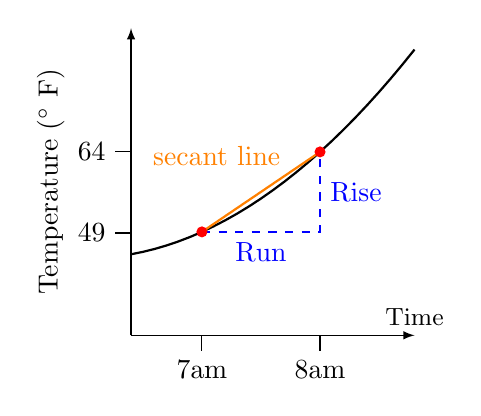
\begin{tikzpicture}[x=12mm,y=13mm,>=latex]
      \uncover<3->{%
        \draw[black,->] (0,0) -- (3,0) node[above] {\small{}Time};
        \draw[black,->] (0,0) -- (0,3);
        % Ticks:
        \draw[thin,black] (0.75,0) -- (0.75,-2mm) node[below] {$7$am};
        \draw[thin,black] (2,0) -- (2,-2mm) node[below] {$8$am};
        \draw[thin,black] (0,1) -- (-2mm,1) node[left] {$49$};
        \draw[thin,black] (0,{0.75+(2+1/2)^2/6}) -- (-2mm,{0.75+(2+1/2)^2/6}) node[left] {$64$};
        \draw[black,thick] plot[domain=0:3] (\x,{0.75+(\x+1/2)^2/6});
        \node[rotate=90] at (-0.85,1.5) {Temperature (${}^{\circ}\ \text{F}$)};
      }
      %
      \uncover<6->{%
        \draw[thick,blue,dashed] (0.75,{0.75+(0.75+1/2)^2/6}) -- node[midway,below] {Run} (2,{0.75+(0.75+1/2)^2/6}) -- (2,{0.75+(2+1/2)^2/6}) node[midway,right] {Rise};
        % 
        \draw[thick,orange] (0.75,{0.75+(0.75+1/2)^2/6}) -- (2,{0.75+(2+1/2)^2/6}) node[near end,left,yshift=2mm] {secant line};
      }
      %
      \uncover<4->{%
        \fill[red] (0.75,{0.75+(0.75+1/2)^2/6}) circle (2pt);
        \fill[red] (2,{0.75+(2+1/2)^2/6}) circle (2pt);
      }
    \end{tikzpicture}
  \end{minipage}


}

\frame{
  \frametitle{Continuing Example}

  Similarly,
  \begin{equation*}
    \left(
      \begin{array}{c}
        \text{{\blue average} rate of} \\
        \text{ change in temp}\\
        \text{between 6am \& 8am}
      \end{array}
    \right)
    = \blue \frac{\text{change in temp}}{\text{time taken}}
  \end{equation*}
  \halfgap

  \alert{Question:}\ \ Suppose temperature at time $t$ given by the
  formula $f(t)=t^2$.  What is the average rate of change of
  temperature from 6am to 8am?
  \begin{center}
    A$= 1$
    \quad 
    B$= 7$ 
    \quad 
    C$= 9$
    \quad 
    D$= 14$
    \quad 
    E$= 28$
    \pause
    \quad 
    \fbox{D} 
  \end{center}
  \gap
  \pause
 
 }
 
 \frame{
   \frametitle{Average Rate of Change}

   Suppose temperature at time $t$ given by the formula $f(t)=t^2$.

   Using a calculator one can find the {\blue average rate of change}
   over shorter and shorter time spans ${\blue\Delta t}$, starting
   at 7am: 

   \begin{table}
     \begin{tabular}{lllllld{2.5}}
       ${\blue\Delta t}$ & $(f(7+{\blue\Delta t})-f(7))/{\blue\Delta t}$
       & \multicolumn{1}{c}{{\blue ave\ rate of change} $^o\text{F}/\text{hr}$}\\
       \toprule
       {\blue1} &$(8^2-7^2)/{\blue 1}$ & 15 \\ \pause
       {\blue0.1} &$(7.1^2-7^2)/{\blue0.1}$ &14.1 \\ \pause
       {\blue0.01} &$(7.01^2-7^2)/{\blue0.01}$& 14.01 \\ \pause
       {\blue0.001} &$(7.001^2-7^2)/{\blue0.001}$& 14.001 \\
       {\blue0.0001} &$(7.0001^2-7^2)/{\blue0.0001}$& 14.0001 \\
       {\blue0.00001} &$(7.00001^2-7^2)/{\blue0.00001}$& 14.00001 \\ \pause
       {\blue 0} & { $(7^2-7^2)/{\blue 0}$} 
       & \multicolumn{1}{c}{$0/{\red 0}$\qquad\qquad{\red arghhhh}}\\
       \bottomrule
     \end{tabular}
     \caption{Average rate of change over various time spans}
   \end{table}
   \vspace*{-1.5em}
   \pause

   What would you {\red guess}\ the {\red exact}\ {\blue
     \emph{instantaneous}\ rate of change} of temperature at precisely
   7am is?\pause\ \  Yes! \fbox{{\blue 14}}.  But how do we get this?\pause
   \ \ Answer: it is a {\red limit}!
 
}

\frame{
   \frametitle{Instantaneous Rate of Change}
   
   What does the limit
   \begin{equation*}
     \lim_{\Delta t \to 0} \frac{f(7+\Delta t) - f(7)}{\Delta t}
   \end{equation*}
   {\red mean} in practice?
   \gap
   \pause 

   Work out the average rate of change over a {\blue very short} time interval.\\
   That is {\blue very nearly} the correct answer.\\
   The shorter the time interval you use, the more accurate you expect
   the answer to be. 
   \gap
   \pause

   To get the {\red exact} answer you would need to take a time interval of zero length.\\
   This leads to the nonsense $\red 0/0.$ So you can't do this.\\
   That is the {\red philosophical} problem. 
   \pause
   \gap

   Mathematical solution: {\red take the limit}.

}


\section{Calculating Slopes}

\frame{
  \frametitle{An Example}
  
  \begin{minipage}{0.5\linewidth}
    A hamster runs along the $x$-axis, so that after $t$ seconds the
    hamster is $t^2$ cm from the origin.  Our goal is to find the
    hamster's speed at time $t=1\ \text{sec}$.
  \end{minipage}
  \begin{minipage}{0.45\linewidth}
    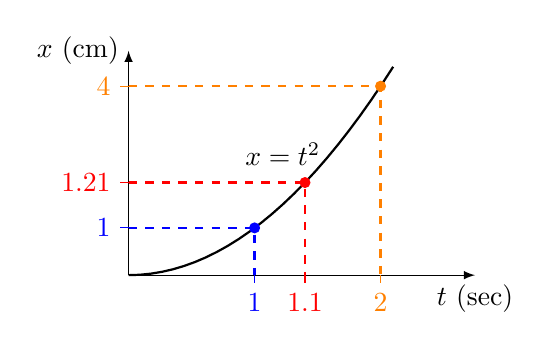
\begin{tikzpicture}[x=16mm,y=6mm,>=latex]
      \draw[black,->] (0,0) -- (2.75,0) node[below] {$t$ (sec)};
      \draw[black,->] (0,0) -- (0,4.75) node[left] {$x$ (cm)};
      % Ticks:
      \draw[thin,blue] (1,0) -- (1,-3pt) node[below] {$1$};
      \draw[thin,blue] (0,1) -- (-3pt,1) node[left] {$1$};
      \uncover<2->{%
        \draw[thin,orange] (2,0) -- (2,-3pt) node[below] {$2$};
        \draw[thin,orange] (0,4) -- (-3pt,4) node[left] {$4$};
      }
      \uncover<3->{%
        \draw[thin,red] (1.4,0) -- (1.4,-3pt) node[below] {$1.1$};
        \draw[thin,red] (0,{1.4^2}) -- (-3pt,{1.4^2}) node[left] {$1.21$};
      }
      % 
      \draw[black,thick] plot[domain=0:2.1] (\x,{(\x)^2});
      \node[left] at (1.6,{1.6^2}) {$x=t^2$};
      \draw[thick,dashed,blue] (0,1) -- (1,1) -- (1,0);
      \fill[blue] (1,1) circle (2pt);
      \uncover<2->{%
        \draw[thick,dashed,orange] (0,4) -- (2,4) -- (2,0);
        \fill[orange] (2,4) circle (2pt);
      }
      \uncover<3->{%
        \draw[thick,dashed,red] (0,{1.4^2}) -- (1.4,{1.4^2}) -- (1.4,0);
        \fill[red] (1.4,{1.4^2}) circle (2pt);
      }
    \end{tikzpicture}
  \end{minipage}

  \begin{align*}
    \uncover<2->{%
      \left(
    \begin{array}{c} 
      \text{average speed from} \\ 
      \text{$t={\blue 1}$ to $t={\orange 2}$}
    \end{array}
    \right) 
    & =  \frac{\text{distance gone}}{\text{time taken}}
    = {{\frac{{\orange 2}^2-{\blue 1}^2}{{\orange 2}-{\blue 1}}}}
    = 3\ \ \text{cm}/\text{sec}
    }
    \\ 
    \uncover<3->{%
    \left(
    \begin{array}{c} 
      \text{average speed from} \\ 
      \text{$t={\blue 1}$ to $t={\red 1.1}$}
    \end{array}\right)  
    & = \frac{\text{distance gone}}{\text{time taken}} 
      =  {{\frac{{\red 1.1}^2-{\blue 1}^2}{{\red 1.1}-{\blue 1}}}}
      % = \frac{1.21-1}{0.1}
      = 2.1\ \text{cm}/\text{sec}
    }
  \end{align*}


}

\frame{
  \frametitle{Example Concluded}

  How do we work out the {\blue exact} speed of the hamster after $1$
  second?
  \smallskip

  \uncover<2->{%
  Plan:
  \begin{itemize}
  \item Find the {\blue average speed} over a short time interval
    ${\red\Delta t}$, then

  \item Take the {\blue limit} as ${\red\Delta t}\to0$.
  \end{itemize}
  }
  \vspace*{-1.5em}

  \begin{align*}
    \uncover<3->{%
    \left(
      \begin{array}{c} 
        \text{average speed from} \\ 
        \text{$t=1$ to $t=1+{\red\Delta t}$}
      \end{array}
    \right) 
    & = \frac{\text{distance gone}}{\text{time taken}}\\ 
    }
    \uncover<4->{%
    & = {{\frac{\left(1+{\red\Delta t}\right)^2\ -\ 1^2}{(1+{\red\Delta t})-1}}}\\ 
    }
    \uncover<5->{%
    & = \frac{(1+2{\red\Delta t}+({\red\Delta t})^2)\ -\ 1}{{\red\Delta t}}\\ 
    }
    \uncover<6->{%
    & = \frac{2{\red\Delta t}+({\red\Delta t})^2}{{\red\Delta t}}\\
    & = 2 + {\red\Delta t}
      }
  \end{align*}

  \uncover<7->{%
  The {\blue limit } of this as ${\red\Delta t}\to0$ is $2$.
  }

  \uncover<8->{%
    Conclusion: At $t=1$ sec, the {\blue exact} speed of the hamster is $2$ cm/sec.
  }
 
  % {\Huge\red\Smiley} \ We have just calculated the.... \pause {\blue instantaneous {\red RAT} of change !}


}


\frame{
  \frametitle{Hamster Summary}

  Soon we will calculate that\ldots

  \begin{empheq}[box=\othermathbox]{align*}
    \text{the {\red exact speed} of the hamster after $t$ seconds is {\red $2t$} cm/sec.}    
  \end{empheq}
  \gap

  Summary:
  \begin{align*}
    {\blue f(t)} 
    &{\blue=  t^2} 
      = \text{{\blue distance} in cm of hamster from origin after $t$ seconds}\\
    & \ \ \text{(a function that gives the distance the hamster has traveled at time $t$)}\\[0.5em]
    %
    {\red f'(t)} 
    &{\red= 2t} 
      = \text{{\red speed} of hamster in cm/sec after $t$ seconds}\\
    & \ \ \text{(called the {\red derivative} of $\blue t^2$
  because it can be {\red derived} or {\red obtained}}\\[-0.5em]
    & \ \ \text{from the function ${\blue t^2}$)} 
  \end{align*}
  \vspace*{-1em}
  \pause

  \alert{Question:}\ \ How many cm had the hamster run by the time its {\red speed} was {\red 8} cm/sec?
  \begin{center}
    A$= 4$
    \quad 
    B$ = 8$
    \quad 
    C$ = 16$
    \quad 
    D$ = 32$
    \quad 
    E$ = 64$
    \quad
    \pause
    \fbox{C}
  \end{center}

}


\frame{
  \frametitle{Exact Hamster Speed}
  Now we calculate that\ldots
  \begin{empheq}[box=\othermathbox]{align*}
    \text{the {\red exact speed} of the hamster after $t$ seconds is {\red $2t$} cm/sec.}    
  \end{empheq}
  \vspace*{-0.5em}

  \uncover<2->{%
  Do this as before: working out the {\blue average speed} over a short time
  interval ${\red\Delta t}$ and taking the {\blue limit} as
  ${\red\Delta t}\to0$ 
  }
  \vspace*{-1em}

  \begin{align*}
    \uncover<3->{%
    \left(
      \begin{array}{c} 
        \text{average speed from} \\ 
        \text{$t$ to $t+{\red\Delta t}$}
      \end{array}
    \right) 
    & = \frac{\text{distance gone}}{\text{time taken}}\\ 
    }
    \uncover<4->{%
    & = {{\frac{\left(t+{\red\Delta t}\right)^2\ -\ t^2}{(t+{\red\Delta t})-t}}}\\ 
    }
    \uncover<5->{%
    & = \frac{(t^2+2t{\red\Delta t}+({\red\Delta t})^2)\ -\ t^2}{{\red\Delta t}}\\ 
    }
    \uncover<6->{%
    & = \frac{2t{\red\Delta t}+({\red\Delta t})^2}{{\red\Delta t}}\\
    & = 2t + {\red\Delta t}
      }
  \end{align*}

  \uncover<7->{%
    The {\blue limit}\ of this as ${\red\Delta t}\to0$ is $2t$.
  }
  % \\
  % \fbox{ So after {\purple t} seconds the {\blue exact} speed of the hamster is $2{\purple t}$ cm/sec.}
 
}

\frame{
  \frametitle{Hamster Questions!}
  
  After $t$ seconds, the hamster is $f(t)=t^2$ cm from origin.

  {\red(1)} What is the {\blue exact} speed (in cm/sec) of the hamster
  at $t=2$?
  \begin{center}
    A$=1$
    \quad 
    B$=2$ 
    \quad 
    C$=4$ 
    \quad 
    D$=6$
    \quad 
    E$=8$
    \quad 
    \pause
    \fbox{C}
  \end{center}
  \medskip
  \pause

  {\red(2)} What is the {\blue exact} speed (in cm/sec) of the hamster
  at $t=4$?
  \begin{center}
    A$=1$
    \quad 
    B$=2$ 
    \quad 
    C$=4$ 
    \quad 
    D$=6$
    \quad 
    E$=8$
    \quad 
    \pause
    \fbox{E}
  \end{center}
  \medskip
  \pause

  {\red(3)} What is the {\blue average} speed (in cm/sec) of the hamster
  from $t=2$ to $t=4$ seconds?
  \begin{center}
    A$=1$
    \quad 
    B$=2$ 
    \quad 
    C$=4$ 
    \quad 
    D$=6$
    \quad 
    E$=8$
    \quad 
    \pause
    \fbox{D}
  \end{center}
  \medskip
  \pause

  Does this make sense?

}

\section{Understanding Derivatives}

\frame{
  \frametitle{Graphical Approach}

  \begin{minipage}{0.5\linewidth}
    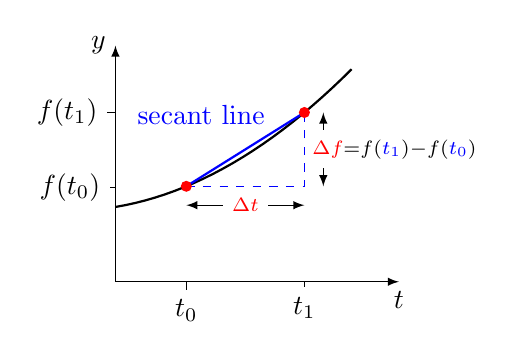
\begin{tikzpicture}[x=12mm,y=12mm,>=latex]
        \draw[black,->] (0,0) -- (3,0) node[below] {$t$};
        \draw[black,->] (0,0) -- (0,2.5) node[left] {$y$};
        % Ticks:
        \draw[thin,black] (0.75,0) -- (0.75,-3pt) node[below] {$t_0$};
        \draw[thin,black] (2,0) -- (2,-2pt) node[below] {$t_1$};
        \draw[thin,black] (0,1) -- (-2pt,1) node[left] {$f(t_0)$};
        \draw[thin,black] (0,{0.75+(2+1/2)^2/6}) -- (-3pt,{0.75+(2+1/2)^2/6}) node[left] {$f(t_1)$};
        \draw[black,thick] plot[domain=0:2.5] (\x,{0.75+(\x+1/2)^2/6});
      %
        \draw[thick,blue] (0.75,{0.75+(0.75+1/2)^2/6}) -- (2,{0.75+(2+1/2)^2/6}) node[near end,left,yshift=2mm] {secant line};
        \draw[thin,black,<->] (0.75,{0.75+(0.75+1/2)^2/6-0.2}) -- (2,{0.75+(0.75+1/2)^2/6-0.2}) node[midway,red,fill=white] {$\scriptstyle\Delta t$};
        \draw[thin,black,<->] (2.2,{0.75+(0.75+1/2)^2/6}) -- (2.2,{0.75+(2+1/2)^2/6}) node[midway,fill=white,right,xshift=-0.75em] {$\scriptstyle{\red\Delta f}=f({\blue t_1})-f({\blue t_0})$};
        \draw[thin,blue,dashed] (0.75,{0.75+(0.75+1/2)^2/6}) -- (2,{0.75+(0.75+1/2)^2/6}) -- (2,{0.75+(2+1/2)^2/6});
        % 
      %
        \fill[red] (0.75,{0.75+(0.75+1/2)^2/6}) circle (2pt);
        \fill[red] (2,{0.75+(2+1/2)^2/6}) circle (2pt);
    \end{tikzpicture}
  \end{minipage}
  \hfill
  \parbox{50mm}{%
    ${\red\Delta f}=$ change in $f$ \\
    ${\red\Delta t}=$ change in $t$\\[0.5em]
    \alert{Many ways to say same thing:}\\
    $\begin{array}{l}
       \left(\begin{array}{c} \text{{\blue average} rate of}\\ \text{change of $f$}\end{array}\right)  = \dfrac{\text{change in $f$}}{\text{change in $t$}}\\
       = \dfrac{\red \Delta f}{\red\Delta t}\\
       =  \text{slope of {\blue secant line}}
       = \dfrac{f({\blue t_1})-f({\blue t_0})}{{\blue t_1}-{\blue t_0}}
     \end{array}$
   }
   \pause

   The derivative is defined to be
   \begin{equation*}
     \lim_{\Delta t\to0} \left(\frac{\red\Delta f}{\red\Delta t}\right) 
     = \frac{df}{dt}
   \end{equation*}
   \pause

   Idea: As $t_1$ moves closer to $t_0$ the secant line approaches the {\blue tangent line}  at $t_0$.
   This is the line with the {\blue same slope} as the graph at $t_0$.

   % \fbox{{\red Let's watch a movie }} \qquad\qquad  No, not  {\blue The Bourne Identity}  :(\\

   % http://www.youtube.com/watch?v=AdQG2iSLDjA\\
   % http://www.youtube.com/watch?v=s3q8D79bjiE\&feature=related
}



\frame{
  \frametitle{Understanding Derivatives}

  There are many ways to {\blue think} about derivatives.  You {\blue
    need} to understand these to apply to problems. 
  \gap
  \gap 

  \begin{minipage}{0.35\linewidth}
    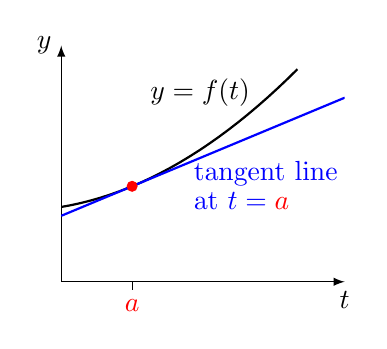
\begin{tikzpicture}[x=12mm,y=12mm,>=latex]
        \draw[black,->] (0,0) -- (3,0) node[below] {$t$};
        \draw[black,->] (0,0) -- (0,2.5) node[left] {$y$};
        % Ticks:
        \draw[thin,black] (0.75,0) -- (0.75,-3pt) node[below] {\red$a$};
        % \draw[thin,black] (2,0) -- (2,-2pt) node[below] {$t_1$};
        % \draw[thin,black] (0,1) -- (-2pt,1) node[left] {$f(t_0)$};
        % \draw[thin,black] (0,{0.75+(2+1/2)^2/6}) -- (-3pt,{0.75+(2+1/2)^2/6}) node[left] {$f(t_1)$};
        \draw[black,thick] plot[domain=0:2.5] (\x,{0.75+(\x+1/2)^2/6});
        \begin{scope}
          \clip (0,0) rectangle (3,2.5);
          \draw[blue,thick] plot[domain=0:3] (\x,{(0.75+1/2)*(\x-0.75)/3+0.75+(0.75+1/2)^2/6});
          \node[blue,right] at (1.3,1.15) {tangent line};
          \node[blue,right] at (1.3,0.85) {at $t={\red{}a}$};
          \node[left] at (2.1,2) {$y=f(t)$};
        \end{scope}
      %
      %
        \fill[red] (0.75,{0.75+(0.75+1/2)^2/6}) circle (2pt);
    \end{tikzpicture}
  \end{minipage}
  \hfill
  \parbox{60mm}{%
    slope of {\blue graph} at {\red a}\\
    = slope of {\blue tangent line} \\%\small{\red $\quad\quad^{discuss}$}\\
    = {\purple instantaneous rate of change} of $f$ at ${\red a}$\\
    \\
    $= \left(
      \begin{array}{l}
        \text{limit of average rate of change } \\ 
        \text{of $f$ over shorter and shorter}\\
        \text{ time intervals starting at\ {\red$a$}}
      \end{array}
    \right)$\\
    \\
    $=$ limit of slopes of secant lines\\
    $= f'({\red a})\ =\ \left. \dfrac{df}{dt}\right|_{t={\red a}}$
  }

}

\frame{
  \frametitle{Summary}

  \begin{itemize}
  \item[$\red \bullet$] How fast something changes $=$ {\blue rate of
      change}
    \bigskip

  \item[$\red \bullet$] {\red Instantaneous} {\blue rate of change} is
    the {\redgreen limit} of the average rate of change over shorter
    and shorter time spans. This gets around the ${\red 0/0}$
    problem. 
    \bigskip

  \item[$\red \bullet$] {\blue speed} $=$ rate of change of distance traveled.
    \bigskip

  \end{itemize}

}

\frame{
  \frametitle{Examples}
  \begin{minipage}{0.5\linewidth}
    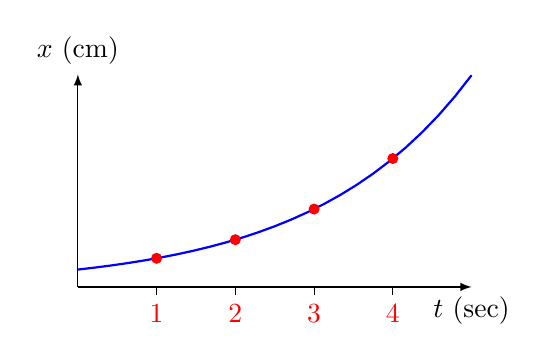
\begin{tikzpicture}[x=10mm,y=6mm,>=latex]
      \draw[thin,black,->] (0,0) -- (5,0) node[below] {$t$ (sec)};
      \draw[thin,black,->] (0,0) -- (0,4.5) node[above] {$x$ (cm)};
      \draw[thick,blue] plot[domain=0:5] (\x,{exp((\x-2)/2)});
      \foreach \x in {1,2,3,4}
      {
        \draw[thin,black] (\x,0) -- (\x,-3pt) node[below] {$\red\x$};
        \fill[red] (\x,{exp((\x-2)/2)}) circle (2pt);
      }
    \end{tikzpicture}
  \end{minipage}
  \hfill
  \begin{minipage}{0.4\linewidth}
    The graph shows the distance from the origin in cm after $t$
    seconds of a hamster.  Which of the numbers below is the largest? 
    \bigskip
    
    \textbf{Hint:}\ Speed is a slope!
  \end{minipage}

  \begin{align*}
    \text{A} & = \text{speed of the hamster at $t=1$} \\
    \text{B} & = \text{speed of the hamster at $t=2$} \\
    \text{C} & = \text{speed of the hamster at $t=3$} \\
    \text{D} & = \text{average speed of the hamster between $t=2$ and $t=3$} \\
    \text{E} & = \text{average speed of the hamster between $t=3$ and $t=4$}
  \end{align*}
  \pause
  % \alert{Answer:}\ \fbox{E}

}

\end{document}

\frame{
  \frametitle{Practical Meaning}

  Our goal is that you understand the {\blue practical meaning} of the
  derivative in various situations. 
  \gap
  \pause

  \begin{align*}
    f({\blue t})
    & = \text{temperature in ${}^{\circ}\ \text{F}$ at ${\blue t}$ hours after midnight}\\
    f({\blue 7})
    & = {\orange 48}\ 
      \text{means the temperature at {\blue 7}am was ${\orange 48}^\circ\ \text{F}$}\\
    f{\red '}({\blue 7})
    & ={\orange 3}\ 
      \text{means}\
      \text{at {\blue 7}am the temperature was rising at a rate of
      ${\orange 3}^{\circ}\ \text{F}/\text{hr}$} \\
    f{\red '}({\blue 9})
    & ={\orange -5}\ 
      \text{means}\ 
      \text{at {\blue 9}am the temperature was {\red falling} at a
      rate of ${\orange 5}^{\circ}\ \text{F}/\text{hr}$}\\ 
    & \hspace*{0.75in}\text{or {\red rising} at a rate of ${\orange
      -5}^{\circ}\ \text{F}/\text{hr}$}
  \end{align*}
  \gap
  \pause
  \begin{align*}
    g({\blue t})
    & = \text{distance from origin in cm of hamster on $x$-axis  after $\blue t$ seconds}\\
    g({\blue 7})
    & ={\orange 3}\
      \text{means after ${\blue 7}$ seconds hamster was ${\orange 3}$ cm from origin}\\
    g{\red '}({\blue 9})
    & ={\orange -5}\
    \text{means after {\blue 9} seconds our furry friend was running {\blue towards}}\\ 
    & \hspace*{0.25in}\text{the origin at a speed of ${\orange 5}\ \text{cm}/\text{sec}$}
  \end{align*}
}

\frame{
  \frametitle{Another Context}
  
  Suppose $f({\blue t})=$ temperature of oven in ${}^{\circ} \text{C}$
  after $t$ minutes.
  \smallskip

  What do $f(3)=20$ and $f{\red '}(3)=15$ mean?
  \begin{itemize}
  \item[A] After $20$ minutes the oven was at $3^{\circ}\ \text{C}$ and heating up at a rate of $15^{\circ}\ \text{C}/\text{min}$

  \item[B] After $3$ minutes oven temperature was $15^{\circ}\ \text{C}$ and cooling down at a rate to $20^{\circ}\ \text{C}/\text{min}$ 

  \item[C] The oven was heating up at rate of $3^{\circ}\ \text{C}/\text{min}$ after 15 minutes and also after 20 minutes

  \item[D] After 3 minutes the oven was at $20^{\circ}\ \text{C}$ and heating up at a rate of $15^{\circ}\ \text{C}/\text{min}$ 

  \item[E] None of the above

  \end{itemize}
  \pause
  \alert{Answer:}\ \fbox{D}

}

\frame{
  \frametitle{Yet Another Context}

  Now suppose $f(t)=$ the population of the ancient city of Lyrad in
  year $t$.  %{\blue C.E.} = {\blue C}urrent {\blue E}ra
  We are told that  $f(1550) = 1820$ and $f{\red '}(1650) = 1100$.
  Which of the following is true?

  \begin{itemize}
  \item[A] In 1550, the population was 1820 and rising at a rate of 1100 people per year

  \item[B] In 1650, the population was 1100 more than in 1550

  \item[C] In 1650, Lyrad contained 1100 people

  \item[D] In 1550, there were 1820 people in Lyrad, and by 1650 this had increased to 2920

  \item[E] None of above
  \end{itemize}
  \pause

  \alert{Answer:}\ \fbox{E}
}


\frame{
  \frametitle{Context: Mathematics}

  Suppose $f(0)=50$ and $f(10)=70$.  Which of the following is true?

  \begin{itemize}
  \item[A] For all $t$ between $0$ and $10$, the derivative is $f{\red'}(t)=2$

  \item[B] $f{\red'}(0)=2$

  \item[C] It is possible that $f{\red'}(0)=-8$

  \item[D] It is impossible that $f{\red'}(0)=-8$

  \item[E] None of above

  \end{itemize}
  \pause
  \alert{Answer:}\ \fbox{C}
  \gap 
  \pause

  We'll see later that, for example, that $f(x)=x^2-8x+50$ has $f(0)=50$,
  $f(10)=70$, and $f{\red '}(0)=-8$. 

}




\end{document}

g